\documentclass[letterpaper]{article}

% --- Packages
\usepackage[utf8]{inputenc}
\usepackage[T1]{fontenc}
\usepackage[margin=0.25cm]{geometry}
\usepackage{enumitem}
\usepackage{pdfpages}
\usepackage{multicol}
\usepackage{amsmath}
\usepackage{amssymb}
\usepackage[skip=1pt plus1pt, indent=0pt]{parskip}
\usepackage{enumitem}
\usepackage{graphicx}

% --- Data
\title{Descriptive statistics}
\author{Enrique Calderon}
\date{March 2024}

% --- Graphics path
\graphicspath{ {./img/} }

% --- Custom commands
\makeatletter
\let\thetitle\@title
\let\theauthor\@author
\makeatother
\newcommand{\compconj}[1]{%
    \overline{#1}%
}
\newcommand{\divline}{\noindent\makebox[\linewidth]{\rule{\textwidth}{0.4pt}}}
\newcommand{\taninv}{\tan^{-1}}
 
% Example of image adding
%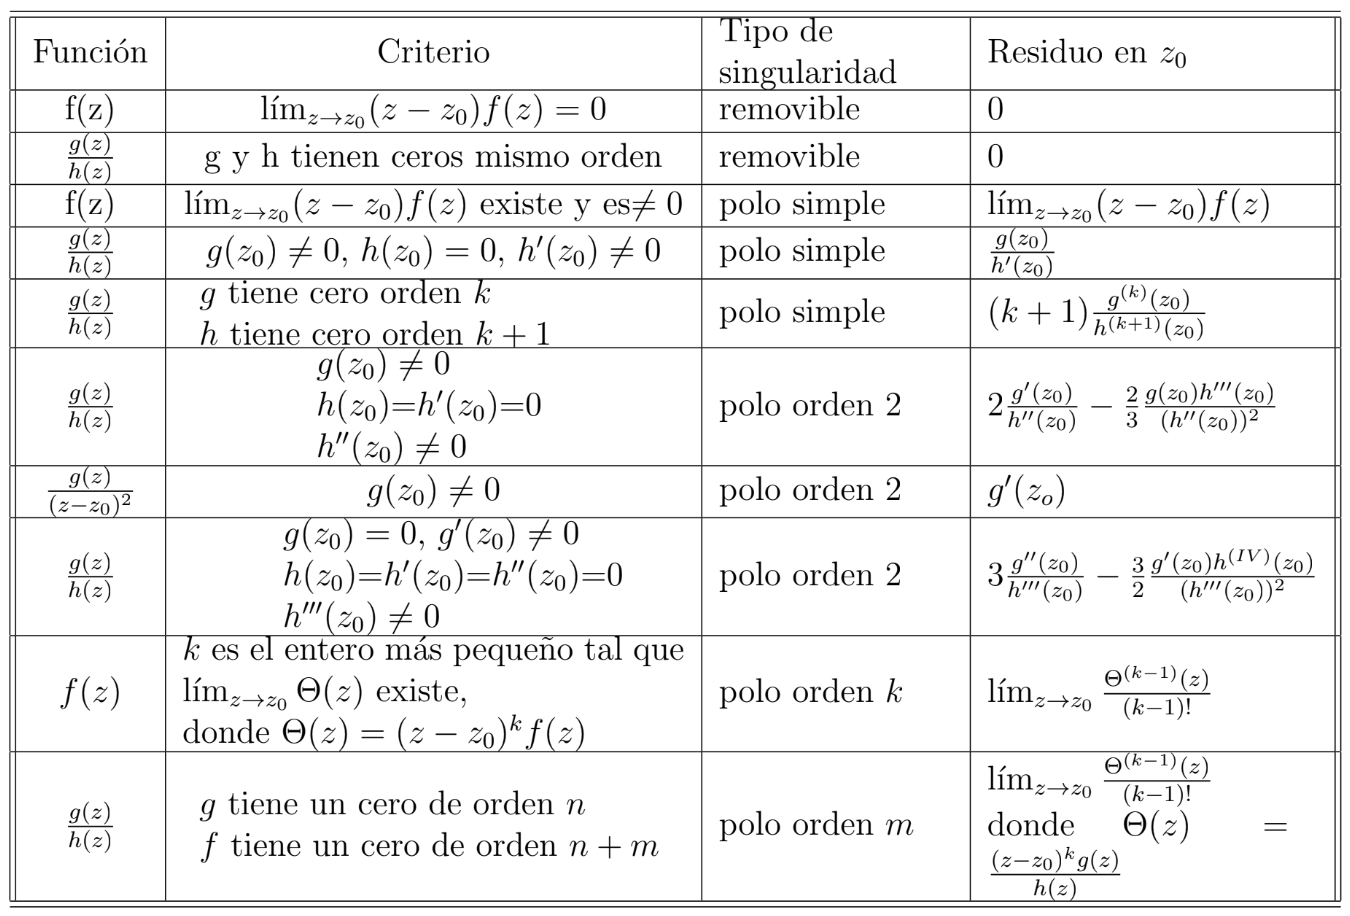
\includegraphics[width=0.8\textwidth]{ResidueTable}

% Remember to add divline between sections

\begin{document}
    \maketitle

    \divline
    \begin{multicols}{2}
        \section{Dispersion measures}

        \subsection{Range}
        
        \[\text{Range } = x_{\text{max}} - x_{\text{min}} \]

        \subsection{Variance}

        \[s^{2} = \frac{\sum_{i=1}^{n} (x_{i} - \hat{x})}{n-1} \]

        \subsection{Standard deviation}

        \[s = \sqrt{s^{2}}\]

        \subsection{Variation coefficient}

        \[\text{C.V. } = \frac{s}{\hat{x}}\]

    \end{multicols}

    \divline
    \begin{multicols}{2}
        \section{Frequency tables}

        \subsection{Number of classes, Sturges's rule}

        \[k = 1 + log_{2}(n)\]

        \subsection{Width of classes}

        \[W = \frac{\text{Range}}{k} = \frac{|x_{\text{max} - x_{\text{min}}|}}{n}\]
        
    \end{multicols}

    \divline
    \begin{multicols}{2}
        \section{Normal distribution}

        \subsection{Empiric rule}

        \begin{align*}
            \text{Value} & \text{ then } & \text{Population quantity} \\
            \hat{x} \pm 1 \cdot s & & 68\% \\
            \hat{x} \pm 2 \cdot s & & 95\% \\
            \hat{x} \pm 3 \cdot s & & 99.9\% \\
        \end{align*}

        \subsection{Percentiles}

        \[Q_{1} = \frac{n+1}{4}\]
        \[Q_{2} = \frac{2(n+1)}{4}\]
        \[Q_{3} = \frac{3(n+1)}{4}\]

        \subsection{Boxplot}

        \[\text{RIC} = Q_{3} - Q_{1}\]
        \[\text{L.I.}  = Q_{1} - 1.5 \cdot \text{RIC}\]
        \[\text{L.S.}  = Q_{3} + 1.5 \cdot \text{RIC}\]

        \subsection{Bias}

        \[\alpha_{3} = \frac{\frac{1}{n} \sum_{i = 1}^{n} (x_{i} - \hat{x})^{3}}{s^{3}}\]

        \subsection{Kurtosis}

        \[\alpha_{4} = \frac{\frac{1}{n} \sum_{i = 1}^{n} (x_{i} - \hat{x})^{4}}{s^{4}}\]

        \subsection{Equation}

        From \(-\infty\) to \(\infty\):

        \[f(x) = \frac{1}{\sigma^{2} \sqrt{2\pi} e^{-\frac{1}{2} \left( \frac{x - \mu}{\sigma^{2}} \right)^{2}} }\]
    \end{multicols}

    \divline
    \begin{multicols}{2}
        \section{Distributions}

        \subsection{Z}

        \[z = \frac{x - \mu}{\sigma}\]

        \[z = \frac{\hat{x} - \mu}{\frac{\sigma}{\sqrt{n}}}\]

        \subsubsection{Standard error}

        \[s_{\hat{x}}  = \frac{s}{\sqrt{n}}\]

        \subsubsection{Table}

        \begin{itemize}
            \item \(z \leq \) : From table
            \item \(z \geq \) : \(1 -\) from table
        \end{itemize}

        

        
    \end{multicols}
\end{document}
